\section{Consultar Recordatorios y Alertas}

Un paciente podrá consultar los recordatorios con los que cuente en ese momento, de esta manera podrá saber cuáles son las medicinas más próximas a tomar, saber su nombre y la dosis.

\subsubsection{Procedimiento}
\begin{enumerate}
	
	\item Da clic en el icono \textbf{Recordatorios} de la pantalla \textbf{Menú Principal}.

		\begin{figure}[!htbp]			\hypertarget{fig:mpPaciente5}{\hspace{1pt}}
		\begin{center}
			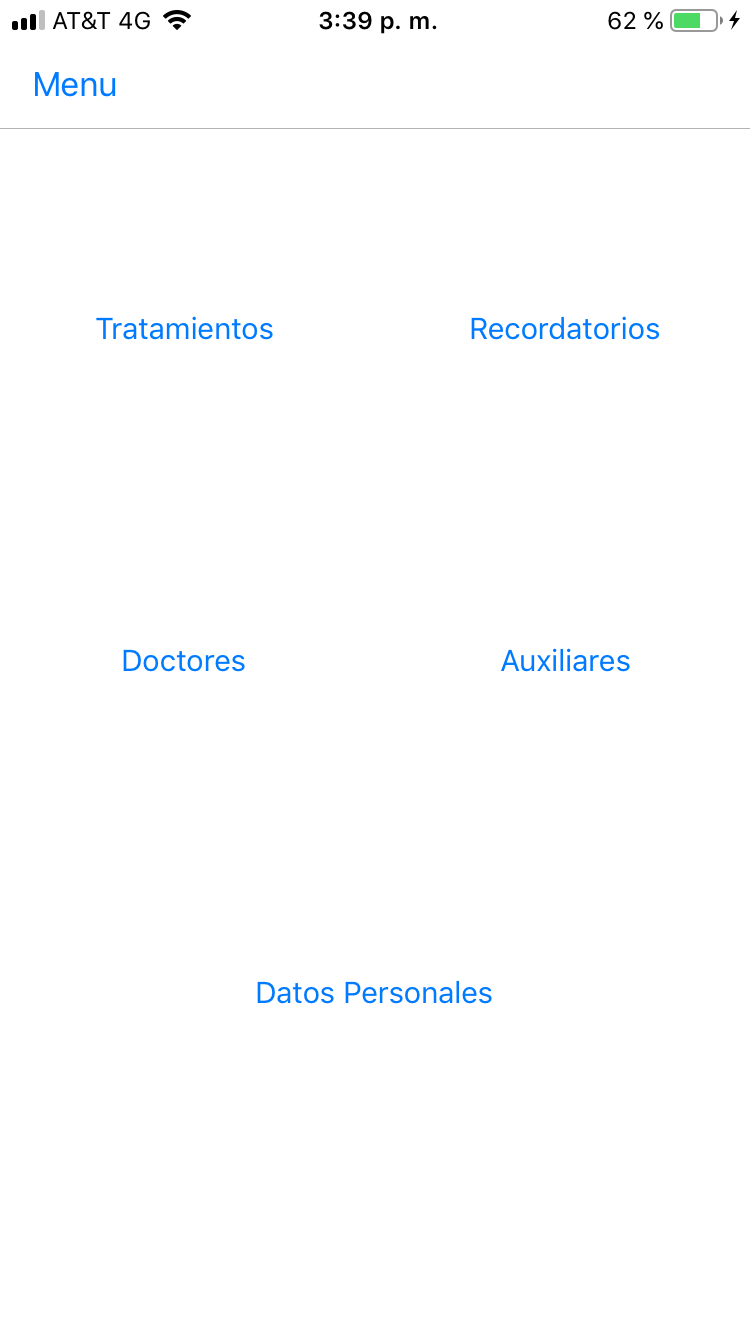
\includegraphics[height=0.4\textheight]{Paciente/ConsultarRecordatorios/images/mpPaciente}
			\caption{Menú Principal Paciente}
			\label{fig:mpPaciente5}
		\end{center}
	\end{figure}

	\item Se mostrará la pantalla \textbf{Recordatorios}. 
	\newpage
	\begin{figure}[!htbp]			
		\hypertarget{fig:Recordatorios}{\hspace{1pt}}
		\begin{center}
			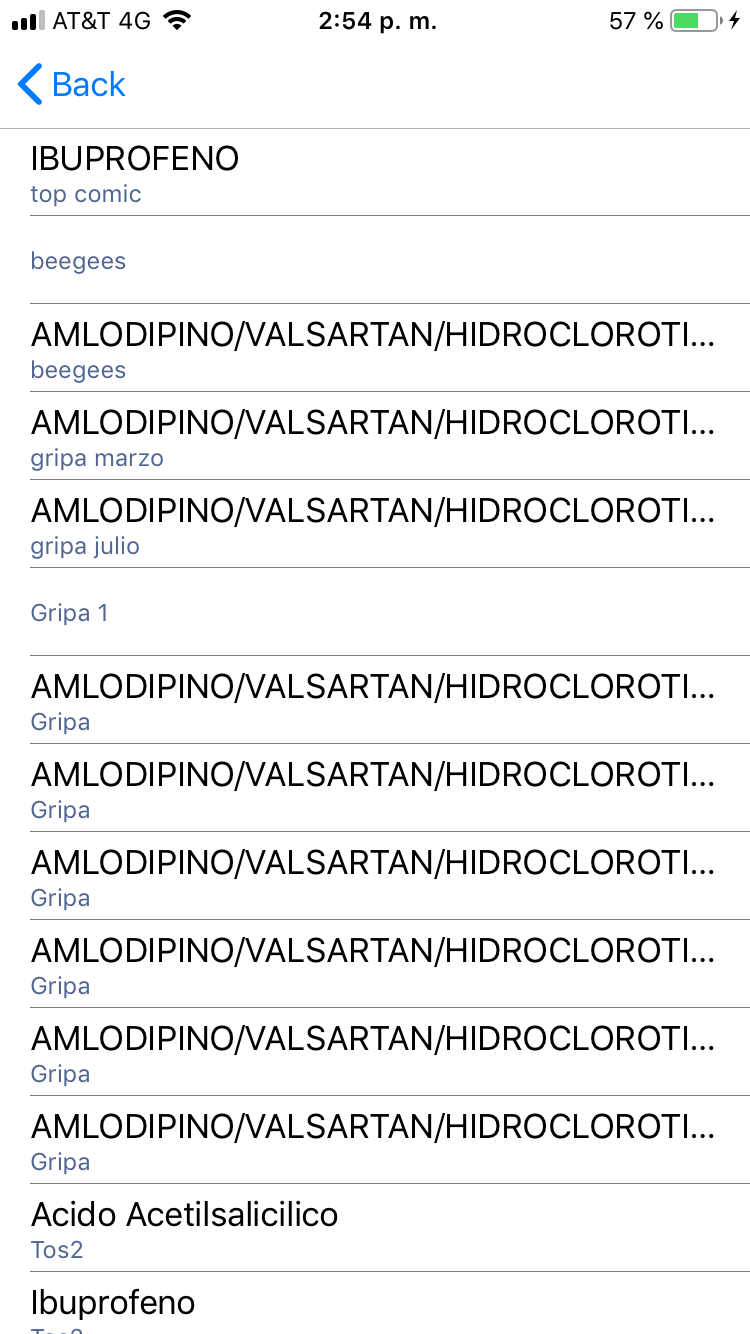
\includegraphics[height=0.4\textheight]{Paciente/ConsultarRecordatorios/images/Recordatorios}
			\caption{Recordatorios}
			\label{fig:Recordatorios}
		\end{center}
	\end{figure}


\end{enumerate}

